\documentclass[12pt]{article}
\usepackage{graphicx}
\usepackage{caption}
\usepackage{subcaption}
\usepackage{float}
%	options include 12pt or 11pt or 10pt
%	classes include article, report, book, letter, thesis

\title{Kuramoto Oscillator}
\author{Tom Wiesing \\ Alee Kazmi}
\date{\today}

\begin{document}
	\maketitle
	\section{Introduction}	
	\subsection{Oscillators}
	Oscillators can be described as a repetitive motion of some measure about a central value which is often the point of equilibrium. This term is most often used in mechanical systems but it must also be noted that oscillations occur in dynamic systems too such as economic graphs, geothermal temperatures across areas and periodic 'firing' of fireflies in nature.
	\begin{figure}[h!]
		\centering
		\begin{subfigure}[h!]{0.3\textwidth}
			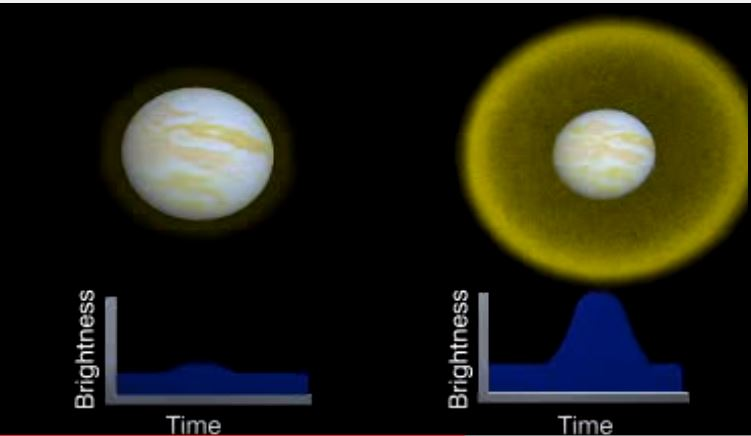
\includegraphics[width=\textwidth]{cepheid}
			\caption{Cepheid Stars that are known to flash occasionally}
			\label{fig:gull}
		\end{subfigure}
		\space\space\space
		\begin{subfigure}[h!]{0.5\textwidth}
			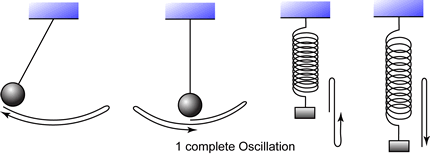
\includegraphics[width=\textwidth]{oscillation}
			\caption{Oscillations}
			\label{fig:gull}
		\end{subfigure}
	\end{figure}
	
	\subsection{Coupling}
	Coupled Oscillation is a slightly more complex form of ordinary oscillators. In these model, the oscillators are connected in such a way that energy is transferred between then. This motion can very well be complex but does not have to be periodic. However, in the bigger scheme of things, every oscillator can be viewed as having a very well defined frequency of its own. Perhaps the simplest example of coupling could be a gear that transmits torque between two shafts that are not collinear. 
	\begin{figure}[h!]
		\centering
		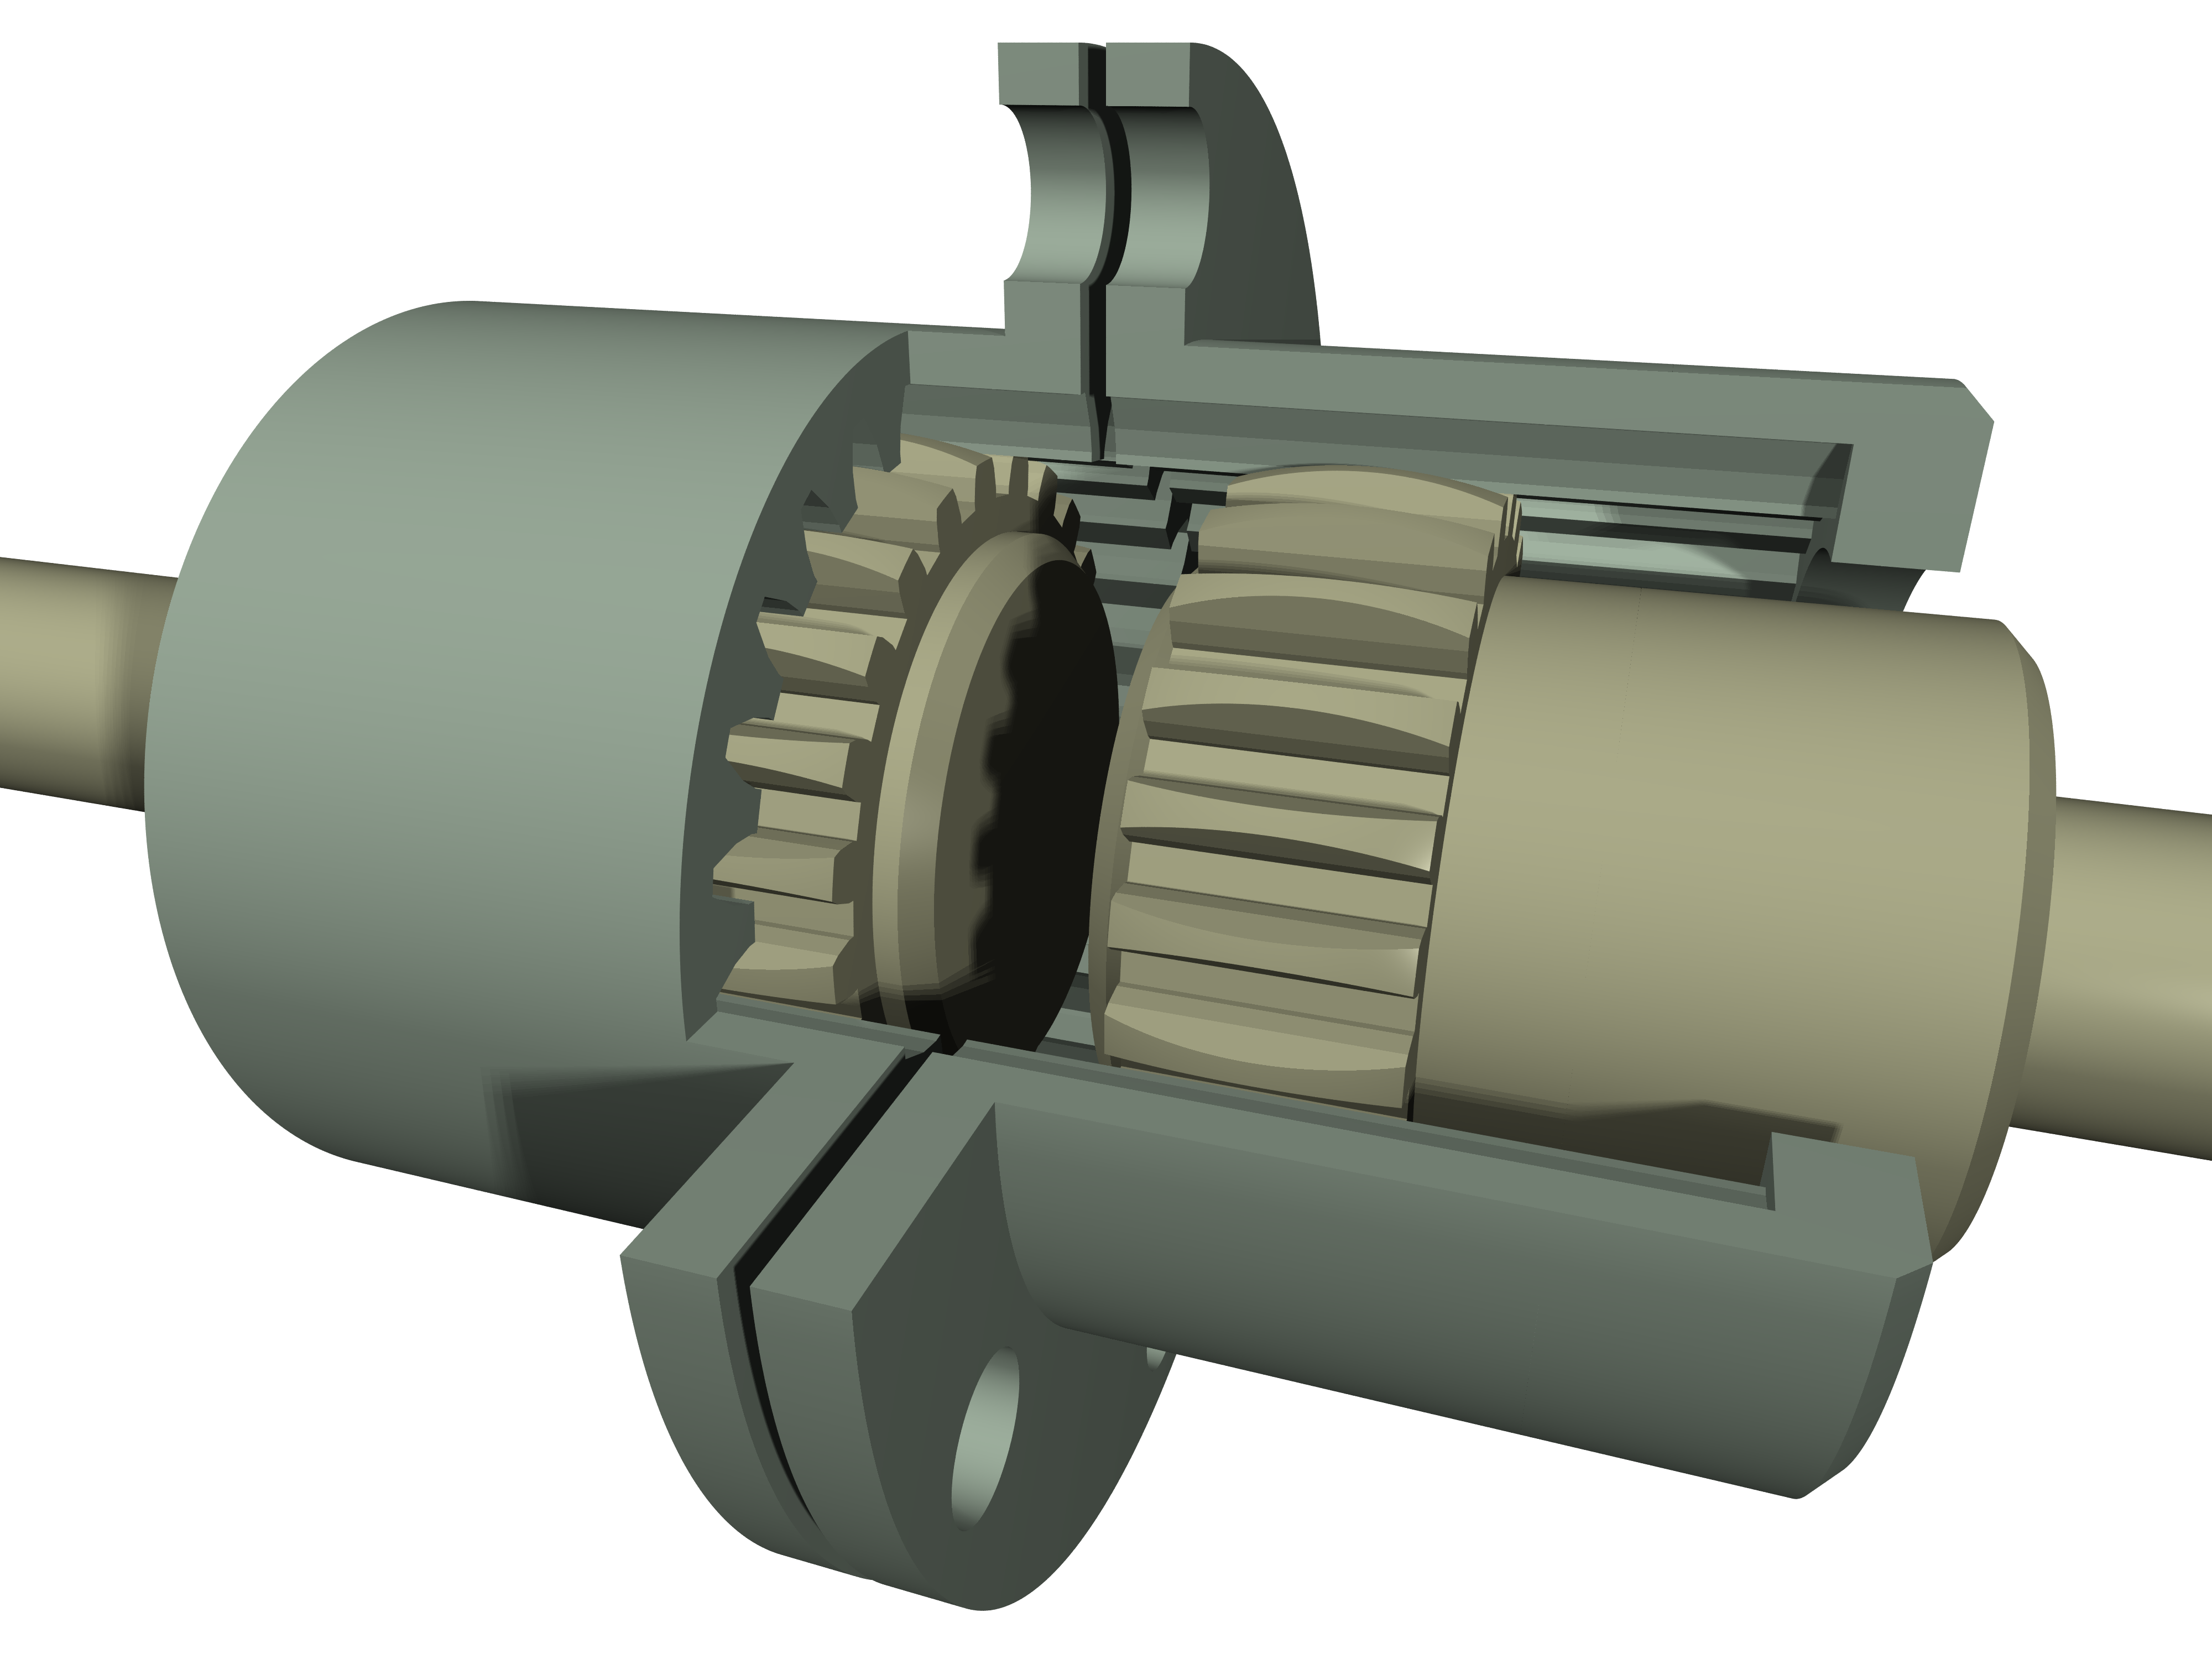
\includegraphics[width=0.5\linewidth]{gear}
		\caption{}
		\label{fig:couple}
	\end{figure}
	\\
	A bit more complex example can be of two pendulums joined together by an energy medium, ie a string.
	\begin{figure}[h!]
\centering
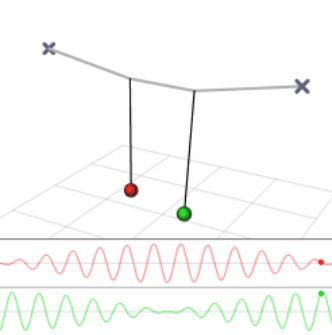
\includegraphics[width=0.5\linewidth]{couple}
\caption{}
\label{fig:couple}
\end{figure}

As we can see in Figure 2, a pendulum only attains its maximum amplitude when the other has its lowest one. This period is achieved after sufficient time has been given to the system to attain synchronization.  

\subsection{Synchronisation}
It should be noted that synchronization can only occur in two ways. The first being if the oscillators have some way of communicating with each other or the second more rarer case where they start at the same exact time. For now we will focus on the first case. Communication can be achieved either by using a medium such as a string between pendulums or even just the intrinsic tendency of natural beings to produce a unison of movement(synchronization) such as fireflies flashing or clapping in a room.

\subsection{Adjacency Matrix and the Network Topology }
Now we move on to define the mathematical tools being used in this project. The Adjacency matrix is a square matrix that is using to represent a finite graph. The elements of the matrix indicate whether pairs of verticies are adjacent or not, ie if they are adjacent they get assigned a value of -1 else 0. This information can be directly retrieved from the topology network graph as follows-:

\begin{figure}[h!]
	\centering
	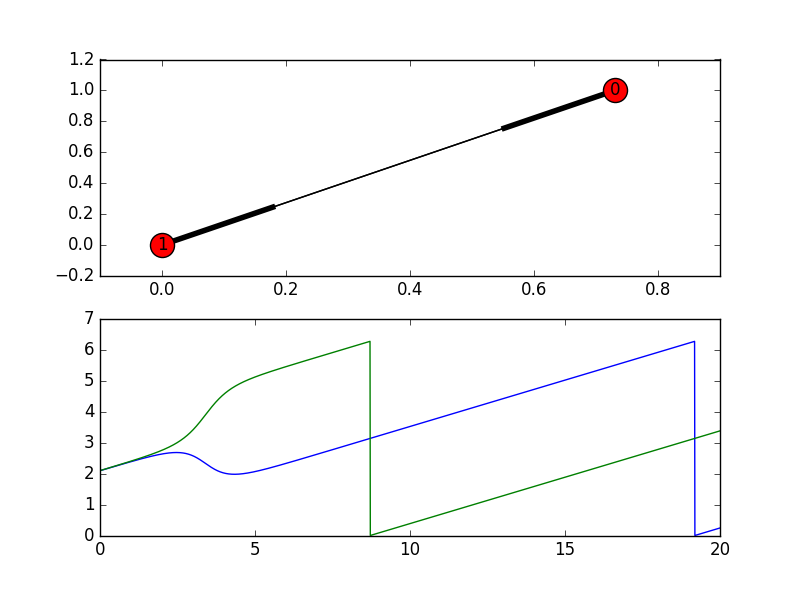
\includegraphics[width=0.5\linewidth]{examplefigure}
	\caption{}
\end{figure}

As we can see, on the top is the topological network containing the vertices of the system and below lies the coupling graphs of the system over time. Over here, we can see that the couples are trying to stay as far away as possible so after the initial unrest there is always a phase difference of 2$\pi$.


\section{Goal}
Our goal for this study is to investigate coupled systems with negative coupling co-efficients. Positive Coupling Coefficients can have expected looking patterns but the results get more interesting for negative ones.

\end{document}